\documentclass[11pt]{article}

\usepackage[margin=1in]{geometry}
\usepackage{amsmath, amssymb, amsthm}
\usepackage{enumitem}
\usepackage{tikz}

\pagestyle{empty}

\begin{document}

\begin{center}
  {\Large\bfseries Weekly Assignment: Graph Theory\\[4pt]
   (Epp~10.1, 10.2, \& 10.3)}
\end{center}

\bigskip

\noindent
Complete each of the following problems.  Show all work and justify your answers.

\bigskip

%% ─────────────────────────────────────────────
\noindent\textbf{Problem 1} (Epp 10.1 \#2). \;
In the graph below, determine whether the following walks are
trails, paths, closed walks, circuits, simple circuits, or just walks.

\begin{enumerate}[label=\textbf{\alph*.},itemsep=2pt]
  \item $v_1 e_2 v_2 e_3 v_3 e_4 v_4 e_5 v_2 e_2 v_1 e_1 v_0$
  \item $v_2 v_3 v_4 v_5 v_2$
  \item $v_4 v_2 v_3 v_4 v_5 v_2 v_4$
  \item $v_2 v_1 v_5 v_2 v_3 v_4 v_2$
  \item $v_0 v_5 v_2 v_3 v_4 v_2 v_1$
  \item $v_5 v_4 v_2 v_1$
\end{enumerate}

\begin{center}
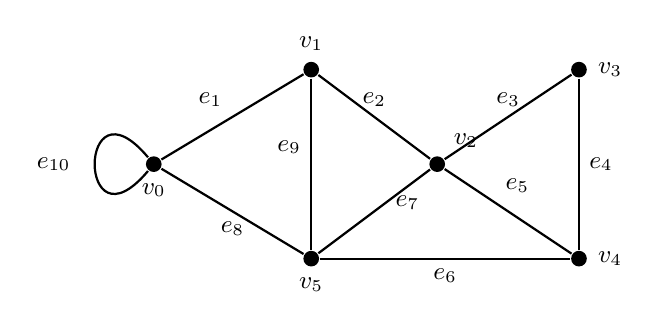
\begin{tikzpicture}[
    vertex/.style={circle, fill=black, inner sep=2pt},
    every node/.style={font=\small},
    thick
  ]
  % Vertices
  \node[vertex, label=below:$v_0$]  (v0) at (0,1.2) {};
  \node[vertex, label=above:$v_1$] (v1) at (2,2.4) {};
  \node[vertex, label=above right:$v_2$] (v2) at (3.6,1.2) {};
  \node[vertex, label=right:$v_3$] (v3) at (5.4,2.4) {};
  \node[vertex, label=right:$v_4$] (v4) at (5.4,0) {};
  \node[vertex, label=below:$v_5$] (v5) at (2,0) {};

  % Edges
  \draw (v0) -- node[above left] {$e_1$} (v1);
  \draw (v1) -- node[above] {$e_2$} (v2);
  \draw (v2) -- node[above] {$e_3$} (v3);
  \draw (v3) -- node[right] {$e_4$} (v4);
  \draw (v2) -- node[above right,pos=0.4] {$e_5$} (v4);
  \draw (v4) -- node[below] {$e_6$} (v5);
  \draw (v2) -- node[right,pos=0.4] {$e_7$} (v5);
  \draw (v0) -- node[below] {$e_8$} (v5);
  \draw (v1) -- node[left,pos=0.4] {$e_9$} (v5);
  % Loop at v0 (drawn large for visibility)
  \draw (v0) to[out=130,in=230,min distance=40pt] node[left=5pt] {$e_{10}$} (v0);
\end{tikzpicture}
\end{center}

\bigskip

%% ─────────────────────────────────────────────
\noindent\textbf{Problem 2} (Epp 10.1 \#5). \;
Consider the following graph.

\begin{center}
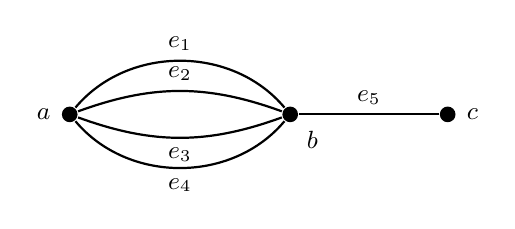
\begin{tikzpicture}[
    vertex/.style={circle, fill=black, inner sep=2pt},
    every node/.style={font=\small},
    thick
  ]
  \node[vertex, label=left:$a$]  (a) at (0,0) {};
  \node[vertex, label=below right:$b$] (b) at (2.8,0) {};
  \node[vertex, label=right:$c$] (c) at (4.8,0) {};

  % Four parallel edges a--b
  \draw (a) to[bend left=50]  node[above] {$e_1$} (b);
  \draw (a) to[bend left=20]  node[above] {$e_2$} (b);
  \draw (a) to[bend right=20] node[below] {$e_3$} (b);
  \draw (a) to[bend right=50] node[below] {$e_4$} (b);
  % One edge b--c
  \draw (b) -- node[above] {$e_5$} (c);
\end{tikzpicture}
\end{center}

\begin{enumerate}[label=\textbf{\alph*.},itemsep=2pt]
  \item How many paths are there from $a$ to $c$?
  \item How many trails are there from $a$ to $c$?
  \item How many walks are there from $a$ to $c$?
\end{enumerate}

\bigskip

%% ─────────────────────────────────────────────
\noindent\textbf{Problem 3} (Epp 10.1 \#18). \;
Is it possible to take a walk around the city whose map is shown
below, starting and ending at the same point and crossing each
bridge exactly once?  If so, how can this be done?

\begin{center}
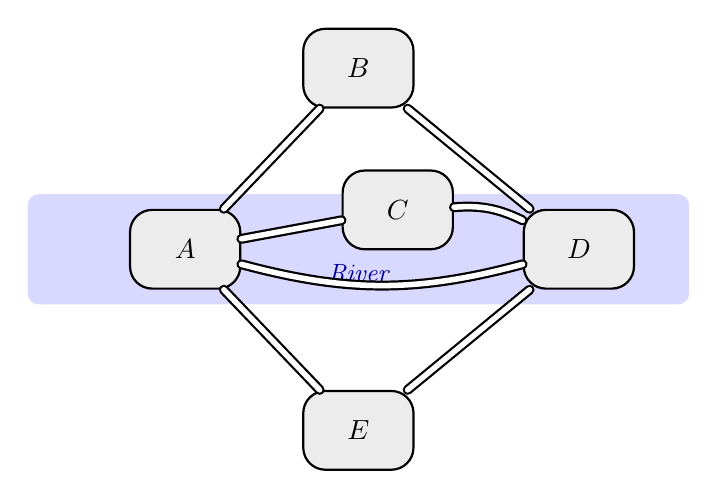
\begin{tikzpicture}[
    region/.style={draw, rounded corners=8pt, minimum width=1.4cm,
                   minimum height=1cm, fill=gray!15, font=\bfseries},
    bridge/.style={double, double distance=2pt, line cap=round},
    thick
  ]
  % River background
  \fill[blue!15, rounded corners=4pt] (-1.2,-0.7) rectangle (7.2,0.7);
  \node[font=\small\itshape, blue!60!black] at (3,-0.3) {River};

  % Regions
  \node[region] (B) at (3,2.3)  {$B$};
  \node[region] (A) at (0.8,0)  {$A$};
  \node[region] (C) at (3.5,0.5){$C$};
  \node[region] (D) at (5.8,0)  {$D$};
  \node[region] (E) at (3,-2.3) {$E$};

  % Bridges
  \draw[bridge] (A) -- (B);
  \draw[bridge] (A) -- (C);
  \draw[bridge] (A) -- (E);
  \draw[bridge] (D) -- (B);
  \draw[bridge] (C) to[bend left=15] (D);
  \draw[bridge] (A) to[bend right=15] (D);
  \draw[bridge] (D) -- (E);
\end{tikzpicture}
\end{center}

\bigskip

%% ─────────────────────────────────────────────
\noindent\textbf{Problem 4} (Epp 10.2 \#5). \;
Find graphs that have the following adjacency matrices.

\medskip

\begin{minipage}[t]{0.45\textwidth}
\centering
\textbf{a.}\quad
$\begin{pmatrix} 1 & 0 & 1 \\ 0 & 1 & 2 \\ 1 & 2 & 0 \end{pmatrix}$
\end{minipage}%
\hfill
\begin{minipage}[t]{0.45\textwidth}
\centering
\textbf{b.}\quad
$\begin{pmatrix} 0 & 2 & 0 \\ 2 & 1 & 0 \\ 0 & 0 & 1 \end{pmatrix}$
\end{minipage}

\bigskip

%% ─────────────────────────────────────────────
\noindent\textbf{Problem 5} (Epp 10.2 \#7). \;
Suppose that for every positive integer~$i$, all the entries in the
$i$th row and $i$th column of the adjacency matrix of a graph
are~0.  What can you conclude about the graph?

\bigskip

%% ─────────────────────────────────────────────
\noindent\textbf{Problem 6} (Epp 10.2 \#9\,b,c). \;
Find each of the following matrix products.

\medskip

\begin{minipage}[t]{0.45\textwidth}
\centering
\textbf{b.}\quad
$\begin{pmatrix} 2 & 0 & 1 \\ 0 & -1 & 0 \end{pmatrix}
\begin{pmatrix} 1 & 3 \\ 5 & -4 \\ -2 & 2 \end{pmatrix}$
\end{minipage}%
\hfill
\begin{minipage}[t]{0.45\textwidth}
\centering
\textbf{c.}\quad
$\begin{pmatrix} -1 \\ 2 \end{pmatrix}
\begin{pmatrix} 2 & 3 \end{pmatrix}$
\end{minipage}

\bigskip

%% ─────────────────────────────────────────────
\noindent\textbf{Problem 7} (Epp 10.3 \#7). \;
Determine whether the simple graphs $G$ and $G'$ below are
isomorphic.  If they are, give a function
$g\colon V(G)\to V(G')$ that defines the isomorphism.
If they are not, give an invariant for graph isomorphism that
they do not share.

\begin{center}
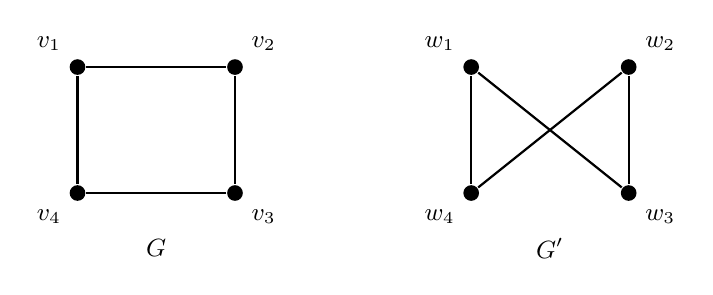
\begin{tikzpicture}[
    vertex/.style={circle, fill=black, inner sep=2pt},
    every node/.style={font=\small},
    thick
  ]
  % Graph G (C4 - cycle)
  \node[vertex, label=above left:$v_1$]  (v1) at (0,1.6) {};
  \node[vertex, label=above right:$v_2$] (v2) at (2,1.6) {};
  \node[vertex, label=below right:$v_3$] (v3) at (2,0) {};
  \node[vertex, label=below left:$v_4$]  (v4) at (0,0) {};

  \draw (v1) -- (v2);
  \draw (v2) -- (v3);
  \draw (v3) -- (v4);
  \draw (v4) -- (v1);

  \node at (1,-0.7) {$G$};

  % Graph G' (K4 - complete graph)
  \begin{scope}[xshift=5cm]
    \node[vertex, label=above left:$w_1$]  (w1) at (0,1.6) {};
    \node[vertex, label=above right:$w_2$] (w2) at (2,1.6) {};
    \node[vertex, label=below right:$w_3$] (w3) at (2,0) {};
    \node[vertex, label=below left:$w_4$]  (w4) at (0,0) {};

     \draw (w2) -- (w3);
    \draw (w4) -- (w1);
    \draw (w1) -- (w3);
    \draw (w2) -- (w4);

    \node at (1,-0.7) {$G'$};
  \end{scope}
\end{tikzpicture}
\end{center}

\bigskip

%% ─────────────────────────────────────────────
\noindent\textbf{Problem 8} (Puzzle). \;
What is the maximum number of edges a simple disconnected graph
with~$n$ vertices can have?  Prove your answer.

\end{document}
